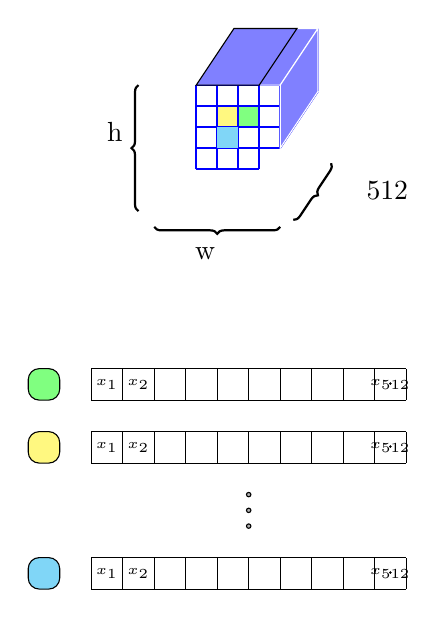
\begin{tikzpicture}[scale=0.8]
	\onslide<1->{
		\renewcommand{\forefillColor}{red!50!white}
		\renewcommand{\borderColor}{white}
		\renewcommand{\toprsidefillcolor}{red!50!white!50}
		\pgfmathsetmacro{\seedx}{0.6}
		\pgfmathsetmacro{\seedy}{1.0}
		\handmadecube{2}{2}{1}{0}{5}

		\draw [
			thick,
			decoration={
				brace,
				mirror,
				raise=0.2cm
			},
			decorate
		] (0,3) -- (0.6,3.9) 
		node [pos=0.1,anchor=north,xshift=-1cm,yshift=-0.4cm] {w}; 

		\draw [
			thick,
			decoration={
				brace,
				mirror,
				raise=0.2cm
			},
			decorate
		] (-2,3) -- (0,3) 
		node [pos=0.1,anchor=north,xshift=2.8cm,yshift=0.5cm] {512};  

		\draw [
			thick,
			decoration={
				brace,
				raise=0.2cm
			},
			decorate
		] (-2,3) -- (-2,5) 
		node [pos=0.1,anchor=north,xshift=-0.5cm,yshift=1.1cm] {h};
		
	}
	
	
	\onslide<3-5>{
		\draw[line width = 0.2mm,step=0.33333,color=blue] (-1,4) grid (0,5);
		\draw [blue,line width = 0.2mm] (-1,4) -- (0,4);
	}
	\onslide<2-5>{
		\fill[green!50!white] (-0.666,4.333) rectangle (-0.333,4.666);

	}
	
	\onslide<5->{
		
		\filldraw[fill=green!50!white, draw=black,rounded corners] (-4,0) rectangle (-3.5,0.5);
		\draw [draw=black,step=0.5] (-3,0) grid (2,0.5);
		\node (x1) at (-2.75,0.25) {\tiny{$x_1$}};
		\node (x2) at (-2.25,0.25) {\tiny{$x_2$}};

		\foreach \x in {-1.75,-1.25,-0.75,-0.25,0.25,0.75,1.25}{
			\node (x2) at (1.75,0.25) {\tiny{$\cdot$}};
		}     
		\node (xn) at (1.75,0.25) {\tiny{$x_{512}$}};
	}
	
	\onslide<5>{
		\draw [blue,line width = 0.2mm] (0,4) -- (0.6,4.9);
		\draw [blue,line width = 0.2mm] (0.6,4.9) -- (0.6,5.9);
		\draw [blue,line width = 0.2mm] (0,5) -- (0.6,5.9);

		\draw [blue,line width = 0.2mm] (-1,5) -- (-0.4,5.9);

		\draw [blue,line width = 0.2mm] (-1,5) -- (-0.4,5.9);

		\draw [blue,line width = 0.2mm] (-0.4,5.9) -- (0.6,5.9);      
		
		\draw  [draw=\borderColor,fill=blue!50] (-1,5) -- (-0.4,5.9) -- (0.6,5.9) -- (0,5)  --cycle ;
		\draw  [draw=\borderColor,fill=blue!50] (0,5)  --(0.6,5.9) -- (0.6,4.9) --(0,4) --cycle ;
	}
	
	
	
	
	\onslide<6>{
		\pgfmathsetmacro\xs{-0.33333};
		\pgfmathsetmacro\ys{0};
		
		\draw[line width = 0.2mm,step=0.33333,color=blue] (-1+\xs,4+\ys) grid (0+\xs,5+\ys);
		\draw [blue,line width = 0.2mm] (-1+\xs,4+\ys) -- (0+\xs,4+\ys);
		
		\draw  [draw=black,fill=blue!50] (-1+\xs,5+\ys) -- (-0.4+\xs,5.9+\ys) -- (0.6+\xs,5.9+\ys) -- (0+\xs,5+\ys)  --cycle ;
		
		%\filldraw[fill=yellow!50!white, draw=black,rounded corners] (-4,0) rectangle (-3.5,0.5);
		
		\fill[yellow!50!white] (-0.666+\xs,4.333+\ys) rectangle (-0.333+\xs,4.666+\ys);
		
	}
	
	\onslide<6->{
		\pgfmathsetmacro\ys{-1cm};
		\filldraw[fill=yellow!50!white, draw=black,rounded corners,yshift=\ys] (-4,0) rectangle (-3.5,0.5);
		\draw [draw=black,step=0.5,yshift=\ys] (-3,0) grid (2,0.5);
		\node[yshift=-0.8cm] (x1) at (-2.75,0.25) {\tiny{$x_1$}};
		\node[yshift=-0.8cm] (x2) at (-2.25,0.25) {\tiny{$x_2$}};

		\foreach \x in {-1.75,-1.25,-0.75,-0.25,0.25,0.75,1.25}{
			\node[yshift=-0.8cm] (x2) at (1.75,0.25) {\tiny{$\cdot$}};
		}     
		\node[yshift=-0.8cm] (xn) at (1.75,0.25) {\tiny{$x_{512}$}};
	}
	
	
	\onslide<7->{
		\filldraw[fill=gray!60!white](-0.5,-1.5)circle(1pt);
		\filldraw[fill=gray!60!white](-0.5,-1.75)circle(1pt);
		\filldraw[fill=gray!60!white](-0.5,-2)circle(1pt);

		\pgfmathsetmacro\ys{-3cm};
		\filldraw[fill=cyan!50!white, draw=black,rounded corners,yshift=\ys] (-4,0) rectangle (-3.5,0.5);
		\draw [draw=black,step=0.5,yshift=\ys] (-3,0) grid (2,0.5);
		\node[yshift=-2.4cm] (x1) at (-2.75,0.25) {\tiny{$x_1$}};
		\node[yshift=-2.4cm] (x2) at (-2.25,0.25) {\tiny{$x_2$}};

		\foreach \x in {-1.75,-1.25,-0.75,-0.25,0.25,0.75,1.25}{
			\node[yshift=-2.4cm] (x2) at (1.75,0.25) {\tiny{$\cdot$}};
		}     
		\node[yshift=-2.4cm] (xn) at (1.75,0.25) {\tiny{$x_{512}$}};
	}
	
	
	\onslide<7>{
		\pgfmathsetmacro\xs{-0.33333};
		\pgfmathsetmacro\ys{-0.33333};
		
		\draw[line width = 0.2mm,step=0.33333,color=blue] (-1+\xs,4+\ys) grid (0+\xs,5+\ys);
		\draw [blue,line width = 0.2mm] (-1+\xs,4+\ys) -- (0+\xs,4+\ys);
		
		%\draw  [draw=black,fill=blue!50] (-1+\xs,5+\ys) -- (-0.4+\xs,5.9+\ys) -- (0.6+\xs,5.9+\ys) -- (0+\xs,5+\ys)  --cycle ;
		
		%\filldraw[fill=cyan!50!white, draw=black,rounded corners] (-4,0) rectangle (-3.5,0.5);
		
		\fill[cyan!50!white] (-0.666+\xs,4.333+\ys) rectangle (-0.333+\xs,4.666+\ys);
		
	}	
\end{tikzpicture}